\documentclass{standalone}
\usepackage{tikz}
\begin{document}
  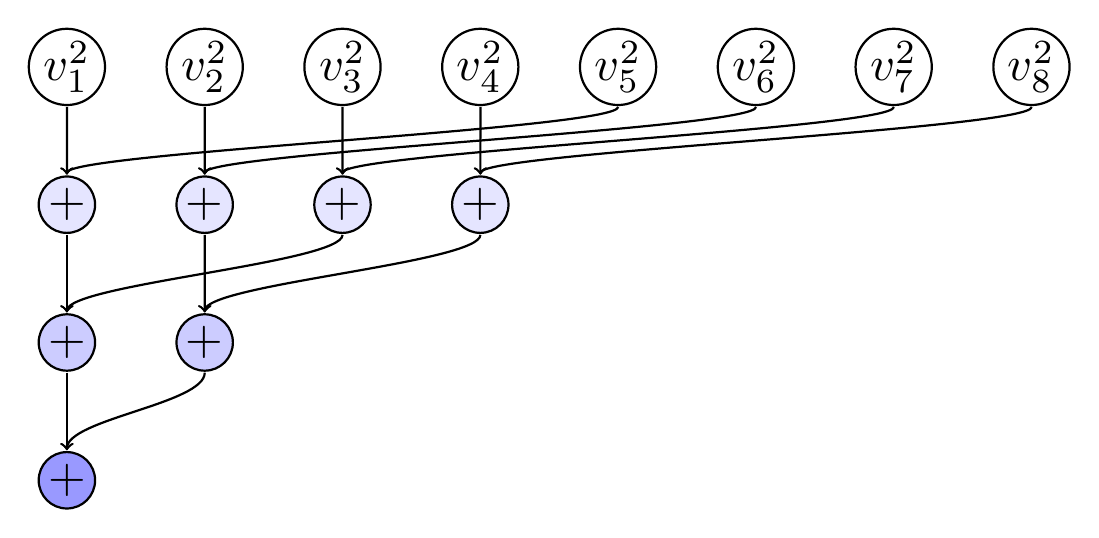
\begin{tikzpicture}[scale=1.75,y=-1cm]
    \tikzset{every node/.style={draw=black,thick,circle,inner sep=0.5pt,scale=1.75}}
    \tikzset{edge/.style={thick}}

    \node (11) at (0, 0) {$v_1^2$};
    \node (12) at (1, 0) {$v_2^2$};
    \node (13) at (2, 0) {$v_3^2$};
    \node (14) at (3, 0) {$v_4^2$};
    \node (15) at (4, 0) {$v_5^2$};
    \node (16) at (5, 0) {$v_6^2$};
    \node (17) at (6, 0) {$v_7^2$};
    \node (18) at (7, 0) {$v_8^2$};

    \node[fill=blue!10] (21) at (0, 1) {$+$};
    \node[fill=blue!10] (22) at (1, 1) {$+$};
    \node[fill=blue!10] (23) at (2, 1) {$+$};
    \node[fill=blue!10] (24) at (3, 1) {$+$};

    \node[fill=blue!20] (31) at (0, 2) {$+$};
    \node[fill=blue!20] (32) at (1, 2) {$+$};

    \node[fill=blue!40] (41) at (0, 3) {$+$};

    \begin{scope}[every path/.style={->}]
       \draw[edge] (11) -- (21);
       \draw[edge] (12) -- (22);
       \draw[edge] (13) -- (23);
       \draw[edge] (14) -- (24);
       \draw[edge] (15) to[out=-90,in=90,looseness=0.1] (21);
       \draw[edge] (16) to[out=-90,in=90,looseness=0.1] (22);
       \draw[edge] (17) to[out=-90,in=90,looseness=0.1] (23);
       \draw[edge] (18) to[out=-90,in=90,looseness=0.1] (24);

       \draw[edge] (21) -- (31);
       \draw[edge] (22) -- (32);
       \draw[edge] (23) to[out=-90,in=90,looseness=0.25] (31);
       \draw[edge] (24) to[out=-90,in=90,looseness=0.25] (32);

       \draw[edge] (31) -- (41);
       \draw[edge] (32) to[out=-90,in=90,looseness=0.5] (41);
    \end{scope}
\end{tikzpicture}
\end{document}
